% !TeX root = ../main.tex
\parindent=0pt
Kotlin Multiplatform Mobile\footnote{\url{https://kotlinlang.org/lp/mobile/}} (KMM) è un framework per lo sviluppo di app iOS e Android basato sul concetto di condivisione della logica applicativa mantenendo lo sviluppo nativo della UX/UI\footnote{User Experience/User Interface}. Consiste in un caso d'uso specifico (e il più diffuso) del framework Kotlin MultiPlatform (KMP), il quale permette di sviluppare il codice in modo agnostico rispetto le piattaforme target e di condividerlo tra differenti piattaforme facendo uso dei tre principali compilatori inclusi nell'ecosistema Kotlin\cite{nagy2022simplifying}:
\begin{itemize}
    \item Kotlin/JVM (Android, Spring, ...)
    \item Kotlin/JS (Web)
    \item Kotlin/Native (iOS, macOS, ...)
\end{itemize}
KMM dipende fortemente dai compilatori Kotlin/JVM (Android) e Kotlin/Native (iOS) e fornisce benefici derivanti sia dallo sviluppo cross-platform che dallo sviluppo nativo:
\begin{itemize}
    \item risparmio di tempo e risorse derivanti dalla condivisione del codice (cross-platform),
    \item alte performance (nativo),
    \item accesso diretto alle funzionalità dei dispositivi hardware senza overhead (nativo).
\end{itemize}
Con il rilascio di Kotlin 1.4 (Agosto 2020), KMM è passato dalla fase "\textit{Experimental}" alla fase "\textit{Alpha}" la quale è considerata come fase "\textit{pre-stable}"\footnote{\url{https://kotlinlang.org/docs/components-stability.html\#stability-levels-explained}} ma è comunque già stato adottato in produzione per lo sviluppo delle proprie applicazioni mobile da tantissime aziende tra le quali è possibile trovare nomi rilevanti come Netflix, VMware e Philips\footnote{\url{https://kotlinlang.org/lp/mobile/case-studies/}}.\\
In base al risultato dell'indagine di mercato svolta nei primi due quadrimestri del 2021\cite{kmm2}, le parti di codice condiviso nelle applicazioni sviluppate con KMM sono:
\begin{itemize}
    \item 85\% Networking
    \item 75\% Data Storage
    \item 70\% Utility (Logging, Analytics, ...)
    \item $\sim$60\% Algoritmi/Computazione
    \item $\sim$55\% State Management
    \item $\sim$50\% Presenters/Controllers/ViewModel
\end{itemize}

\begin{figure}[H]
\centering
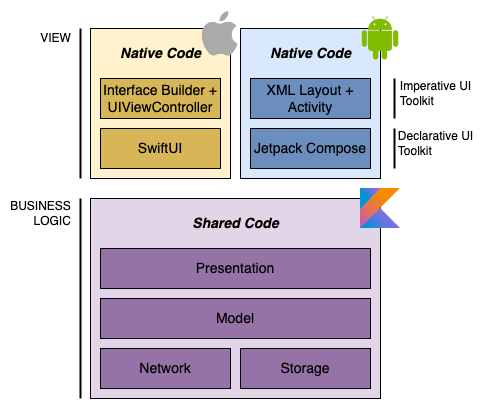
\includegraphics[width=0.8\textwidth]{img/tesi-8-kmm.drawio.png}
\caption{Architettura Kotlin Multiplatform Mobile}
\end{figure}

\section{Kotlin/JVM}
Il compilatore Kotlin/JVM è uno dei due compilatori su cui è basato KMM, utilizzato per la piattaforma Android. Permette di compilare codice Kotlin in bytecode Java (\textit{.class}), il quale può essere eseguito direttamente sulla JVM. Nel caso di Android è necessario un ulteriore passaggio per tradurre il bytecode Java in bytecode Dalvik (\textit{.dex}).

\begin{figure}[H]
\centering
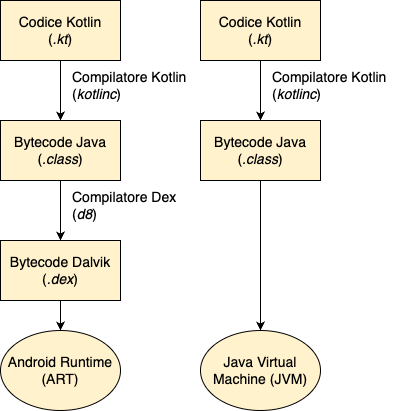
\includegraphics[width=0.55\textwidth]{img/tesi-9-kotlinjvm.drawio.png}
\caption{Fasi di compilazione Kotlin/JVM con piattaforma target Android e JVM}
\end{figure}

\section{Kotlin/Native}
Kotlin/Native è il secondo compilatore su cui è basato KMM e viene utilizzato per la piattaforma iOS. A differenza del compilatore Kotlin/JVM, il compilatore Kotlin/Native è progettato per quelle situazioni dove non è possibile/non si vuole avere una VM come dispositivi embedded e iOS. Per fare ciò include un backend basato su \textit{Low Level Virtual Machine} (LLVM)\footnote{\url{https://llvm.org/}}, ovvero il codice Kotlin viene compilato in binari nativi che possono essere eseguiti senza VM\cite{nagy2022simplifying}. Le piattaforme supportate da Kotlin/Native attualmente sono macOS, iOS, tvOS, watchOS, Linux, Windows (MinGW) e Android NDK\footnote{\url{https://kotlinlang.org/docs/native-overview.html\#target-platforms}} e per ognuna di esse esistono differenti architetture. Nel caso di iOS le differenti architetture supportate da KMM sono \textit{Arm64}, \textit{Arm32} e \textit{x64}.
\begin{figure}[H]
\centering
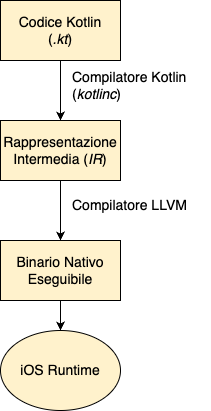
\includegraphics[width=0.28\textwidth]{img/tesi-10-kotlinnative.drawio.png}
\caption{Fasi di compilazione Kotlin/Native con piattaforma target iOS}
\end{figure}
Anche in questo caso sono necessarie due fasi di compilazione: ($i$) il codice Kotlin viene compilato nella \textit{Rappresentazione Intermedia} (IR) LLVM e ($ii$) successivamente compilato nel binario nativo.

\section{Plugin Gradle KMP}
Il plugin Gradle KMP è uno strumento utile per realizzare progetti multiplatform. Fornisce uno specifico DSL\footnote{Domain Specific Language} per definire e configurare i task necessari a compilare il codice condiviso per le relative piattaforme target\footnote{\url{https://kotlinlang.org/docs/multiplatform-dsl-reference.html}}. Al momento la versione latest (stable) del plugin è la \textit{1.6.21}, rilasciata il 19/04/2022\footnote{\url{https://plugins.gradle.org/plugin/org.jetbrains.kotlin.multiplatform/1.6.21}} ma è presente una versione candidata per il rilascio con tag \textit{1.7.0-RC2}.

\begin{listing}[H]
\begin{minted}{kotlin}
plugins {
    kotlin("multiplatform")
    id("com.android.library")
    kotlin("native.cocoapods")
}

kotlin {
    android()
    iosX64()
    iosArm64()
    iosSimulatorArm64()
    
    sourceSets {
        val commonMain by getting {
            dependencies {
                // Dipendenze comuni a Android e iOS
            }
        }

        val androidMain by getting {
            dependencies {
                // Dipendenze specifiche Android
            }
        }

        val iosX64Main by getting
        val iosArm64Main by getting
        val iosSimulatorArm64Main by getting
        val iosMain by creating {
            dependsOn(commonMain)
            iosX64Main.dependsOn(this)
            iosArm64Main.dependsOn(this)
            iosSimulatorArm64Main.dependsOn(this)
            dependencies {
                // Dipendenze specifiche iOS
            }
        }
    }
}
\end{minted}
\caption{Definizione utilizzo Plugin Gradle KMP nel file \textit{build.gradle.kts} del modulo condiviso (Kotlin)}
\end{listing}

\subsection{KMM Android Studio IDE Plugin}
L'IDE\footnote{Integrated Development Environment} Android Studio è costruito su IntelliJ, il quale è uno tra gli IDE più diffusi ed è sviluppato da JetBrains. Tramite il plugin KMM, installabile direttamente dal marketplace integrato in Android Studio o dal sito ufficiale JetBrains\footnote{\url{https://plugins.jetbrains.com/plugin/14936-kotlin-multiplatform-mobile/versions/stable}}, si abilita un insieme di funzionalità a supporto dello sviluppo di codice multiplatform, in particolare:
\begin{itemize}
    \item creazione della struttura e della configurazione base per una nuova applicazione multiplatform,
    \item creazione della struttura e della configurazione base per una nuova libreria multiplatform,
    \item integrazione di moduli multiplatform in applicazioni già esistenti.
\end{itemize}